\documentclass{hitec}
\author{Michael Hansen, Brooke Mosby, Juan Rodr\'iguez, Bailey Smith}
\title{Inverted Pendulum - Cart and Rod}

\usepackage{amsmath}
\usepackage{tikz}
\usepackage{soul}
\settextfraction{.85}

\begin{document}
	\maketitle
	
	\section{Problem Statement}
	You will write code to interact with the provided virtual inverted pendulum. Your
	program should work for a pendulum of arbitrary mass and length. Given the mass and
	length of the pendulum and an initial position, angle, approximate change in position, and
	approximate change in angle, you will move the base of the pendulum horizontally to bring
	the pendulum to within a given tolerance of an unstable steady state of the system. The
	mass and length of the pendulum are constrained in a certain interval. There is also a limit
	on your control, which your code is given at run time.
	
	\[
	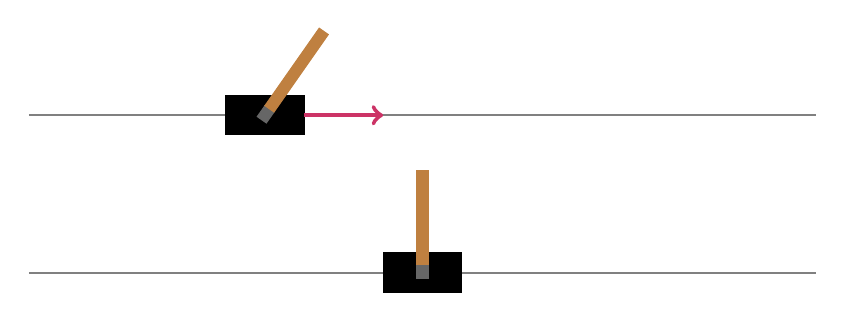
\begin{tikzpicture}
	
	\draw[help lines,thick] (-5,0) -- (5,0);
	\filldraw[black] (-2.5,-.25) -- ++(0,.5) -- ++(1,0) -- ++(0,-.5) -- cycle;
	\begin{scope}[xshift=-2cm,rotate=-35]
	\filldraw[black!60] (-.07,-.07) -- ++(0,.17) -- ++(.14,0) -- ++(0,-.17) -- cycle;
	\filldraw[brown] (-.07,.1) -- ++(0,1.2) -- ++(.14,0) -- ++(0,-1.2) -- cycle;
	\end{scope}
	\draw[ultra thick,->,purple!80] (-1.5,0) -- ++(1,0);
	
	\begin{scope}[yshift=-2cm]
	\draw[help lines,thick] (-5,0) -- (5,0);
	\filldraw[black] (-.5,-.25) -- ++(0,.5) -- ++(1,0) -- ++(0,-.5) -- cycle;
	\filldraw[black!60] (-.07,-.07) -- ++(0,.17) -- ++(.14,0) -- ++(0,-.17) -- cycle;
	\filldraw[brown] (-.07,.1) -- ++(0,1.2) -- ++(.14,0) -- ++(0,-1.2) -- cycle;
	
	\end{scope}
	\end{tikzpicture}
	\]
	
	
	\section{Requirements}
	\begin{enumerate}
		\item 20 points for clearly describing your algorithm for solving the problem
		\item 10 points for making the argument that your algorithm is in some sense optimal
		\item 10 points for fair share of the
		work load
	\end{enumerate}
	
	
	\section{Our Algorithm}
	We used code that we had implemented in the Inverted Pendulum Lab. We are given $M$ (the mass of the cart), $m$ (the mass of the rod), $l$ (the length of the rod), $q_1$, $q_2$, $q_3$, $q_4$ (which are nonnegative weights used in the diagonal of the matrix Q), and $r$ (which is the nonnegative weight making up the matrix R). Along with these parameters, we use the function \texttt{linearized\_init} to construct and return the matrices $A$, $B$, $Q$, and $R$.
	The formulas for the matrices were found from these equations:
	\begin{align}
	F&=M\ddot{x}+b\dot{x}+N                                  \\
	N&=m\ddot{x}+ ml\ddot{\theta}\cos{\theta}-ml\dot{\theta^2}\sin{\theta} \\
	\end{align}
	Which become:
	\begin{align}
	(I + ml^2)\ddot{\theta}-mgl\theta&=ml\ddot{x} \\
	(M+m)\ddot{x}+b\dot{x}-ml\ddot{\theta}&=u     \\
	\end{align}
	With $I=\frac{1}{3}*m*l^2$. So the matrices are:
	\[
	A=
	\begin{bmatrix}
	0 & 1 & 0                              & 0 \\
	0 & 0 & \frac{m^2gl^2}{I(M+m)+Mml^2}  & 0 \\
	0 & 0 & 0                              & 1 \\
	0 & 0 & \frac{mgl(M+m)}{I(M+m)+Mml^2}  & 0
	\end{bmatrix}
	\]
	\[
	B=
	\begin{bmatrix}
	0                           \\
	\frac{I+ml^2}{I(M+m)+Mml^2} \\
	0                           \\
	\frac{ml}{I(M+m)+Mml^2}
	\end{bmatrix}
	\]
	\[
	Q=
	\begin{bmatrix}
	q_1 & 0   & 0   & 0 \\
	0   & q_2 & 0   & 0 \\
	0   & 0   & q_3 & 1 \\
	0   & 0   & 0   & q_4
	\end{bmatrix}
	\]
	\[
	R=
	\begin{bmatrix}
	r
	\end{bmatrix}
	\]
	Next, we implement a function called \texttt{rickshaw} which takes in parameters $tv$ (an array of time values), $X0$ (initial conditions on the state variables), $A$, $B$, $Q$, $R$ (which we get from \texttt{linearized\_init}), and a matrix $P$. $P$ is calculated using \texttt{scipy.linalg.solve\_continuous} \texttt{\_are} which solves the algebraic Riccati equation given $A$, $B$, $Q$, and $R$. \texttt{rickshaw} is a Linear Quadratic Regulator which will calculate and return the optimal control $U$ and the optimal state vector $Z$. This is all done inside our function \texttt{stabilize}.\\\\
	To stabilize the rod on the cart vertically, we first initialize $X0$ using \texttt{env.reset()}. We give it our optimized $q$s and $r$ that will be explained in the next section. We get $Z$ and $U$ using our \texttt{stabilize} function. Then, for each step in time (.02 seconds), we take the observation from \texttt{env.step()} on the first element of $U$, use it to contruct a new $X0$, then call \texttt{stabilize} for a new $U$ and $Z$. $U$ actually calculates the expected optimal controls for the rest of time, however we update after taking each next step. So, we use the first element of $U$ in each iteration.
	
	\section{What Makes it Optimal?}
	\hl{Talk about why LQR is good and what Brooke did to choose parameters}\\
	We chose to use the LQR algorithm because it is like an automated method for us to find the state-feedback controller. So it gives us very efficient feedback gains.
	
	
	
\end{document}